\section{Aufbau und Generierung der Irradiance Map} % (fold)
\label{sec:aufbau_und_generierung_der_irradiance_map}

	\begin{figure}[h]
		\begin{subfigure}[t]{0.33\textwidth}
			\center
			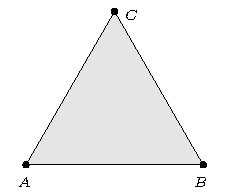
\includegraphics{gg_fig/irr_map_ds-order_1.pdf}
			\caption{\parbox[t]{0.5\textwidth}{Ordnung: $1$ \\ Samples: $3$}}
		\end{subfigure}
		\begin{subfigure}[t]{0.33\textwidth}
			\center
			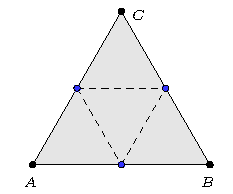
\includegraphics{gg_fig/irr_map_ds-order_2.pdf}
			\caption{\parbox[t]{0.5\textwidth}{Ordnung: $2$ \\ Samples: $6$}}
		\end{subfigure}
		\begin{subfigure}[t]{0.33\textwidth}
			\center
			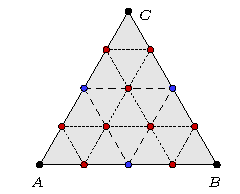
\includegraphics{gg_fig/irr_map_ds-order_4.pdf}
			\caption{\parbox[t]{0.5\textwidth}{Ordnung: $4$ \\ Samples: $15$}}
		\end{subfigure}
		\caption{Die Abbildung zeigt das Schema der Dreieck Irradianc Map Datenstruktur auf einem Dreieck $(A,B,C)$ für verschiedene Ordnungen.}
		\label{fig:scheme-irr-map}
	\end{figure}

	\begin{figure}[h]
		\begin{subfigure}[t]{0.5\textwidth}
			\center
			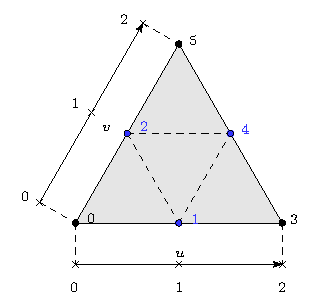
\includegraphics{gg_fig/irr_map_memidx-order_2.pdf}
			\caption{Ordnung: $2$}
		\end{subfigure}
		\begin{subfigure}[t]{0.5\textwidth}
			\center
			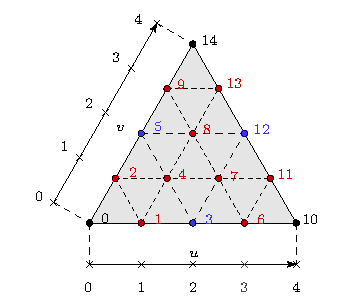
\includegraphics{gg_fig/irr_map_memidx-order_4.pdf}
			\caption{Ordnung: $4$}
		\end{subfigure}
		\caption{Die Abbildung zeigt das Schema der Dreieck Irradianc Map Datenstruktur für verschiedene Ordnungen.}
		\label{fig:scheme-irr-map}
	\end{figure}

	\[
		\func{s}{\SN}{\SN},\qquad s(n)\define \frac{(n+1)(n+2)}{2}
	\]
	\[
		U_n\define \set[u+v\leq n]{(u,v)\in\SN_0^2},\qquad I_n\define \set[i < s(n)]{i\in\SN_0}
	\]
	\[
		\func{m_n}{U_n}{I_n},\qquad m_n(u,v) \define \frac{(u+v)(u+v+1)}{2} + v
	\]
	\[
		\func{m_{n,p}}{U_n}{I_{n\cdot 2^p}},\qquad m_{n,p}(u,v)\define m_{n\cdot 2^p}(u\cdot 2^p,v\cdot 2^p)
	\]

	\medskip
\begin{tcolorbox}[colframe=black,colbacktitle=white,coltitle=black, attach boxed title to top center={yshift=-2mm},enhanced, titlerule=0.1pt, boxrule=0.5pt, arc=5pt,title=Quelltext:\quad Dreieck Irradiance Map Datenstruktur, breakable]
	\lstinputlisting[style=std,language=c++]{code/irr_map.cpp}
\end{tcolorbox}
\medskip

	\begin{figure}[h]
		\begin{subfigure}[b]{0.33\textwidth}
			\center
			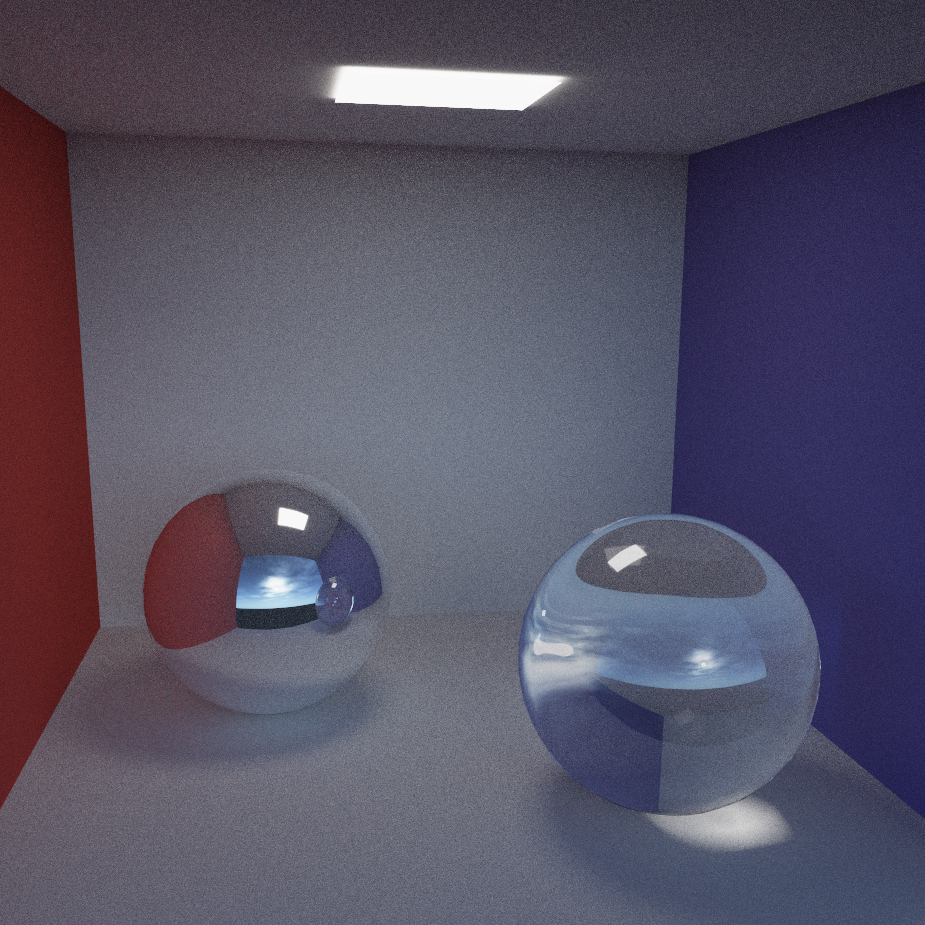
\includegraphics[width=0.95\textwidth]{pic/irrmap-cornell-ref.png}
			\caption{Path Tracing}
		\end{subfigure}
		\begin{subfigure}[b]{0.33\textwidth}
			\center
			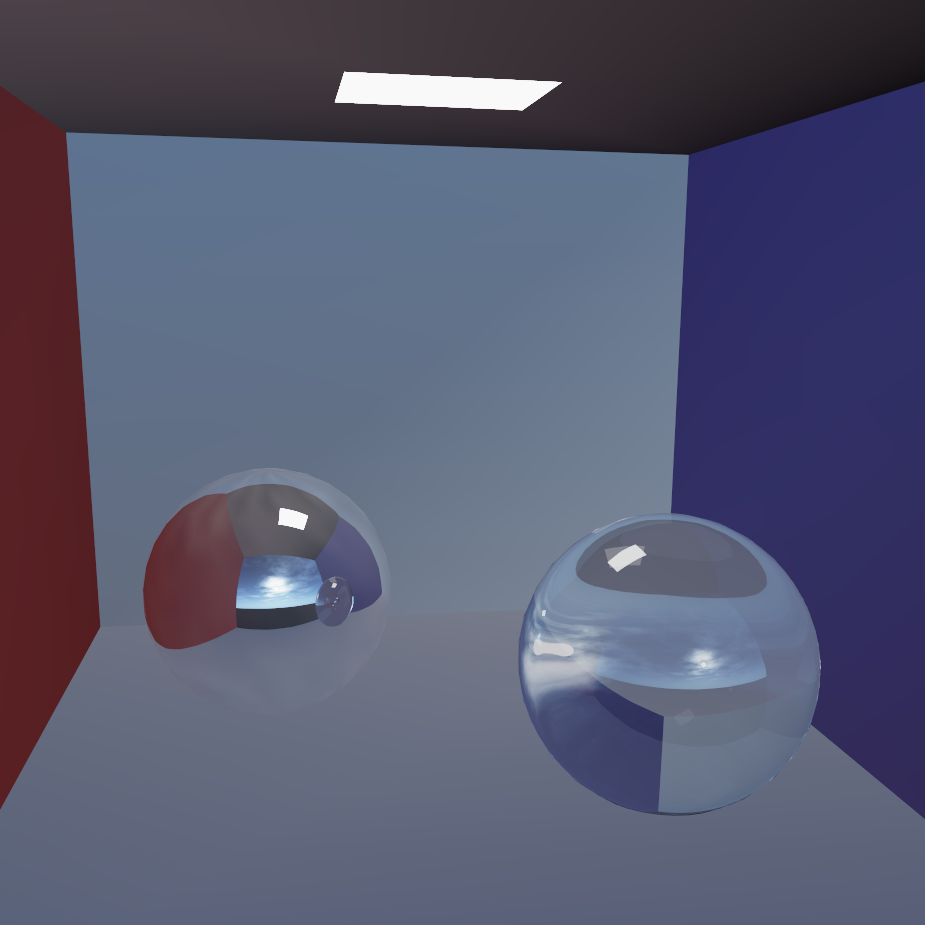
\includegraphics[width=0.95\textwidth]{pic/irrmap-cornell-vmap.png}
			\caption{Vertex Lighting}
		\end{subfigure}
		\begin{subfigure}[b]{0.33\textwidth}
			\center
			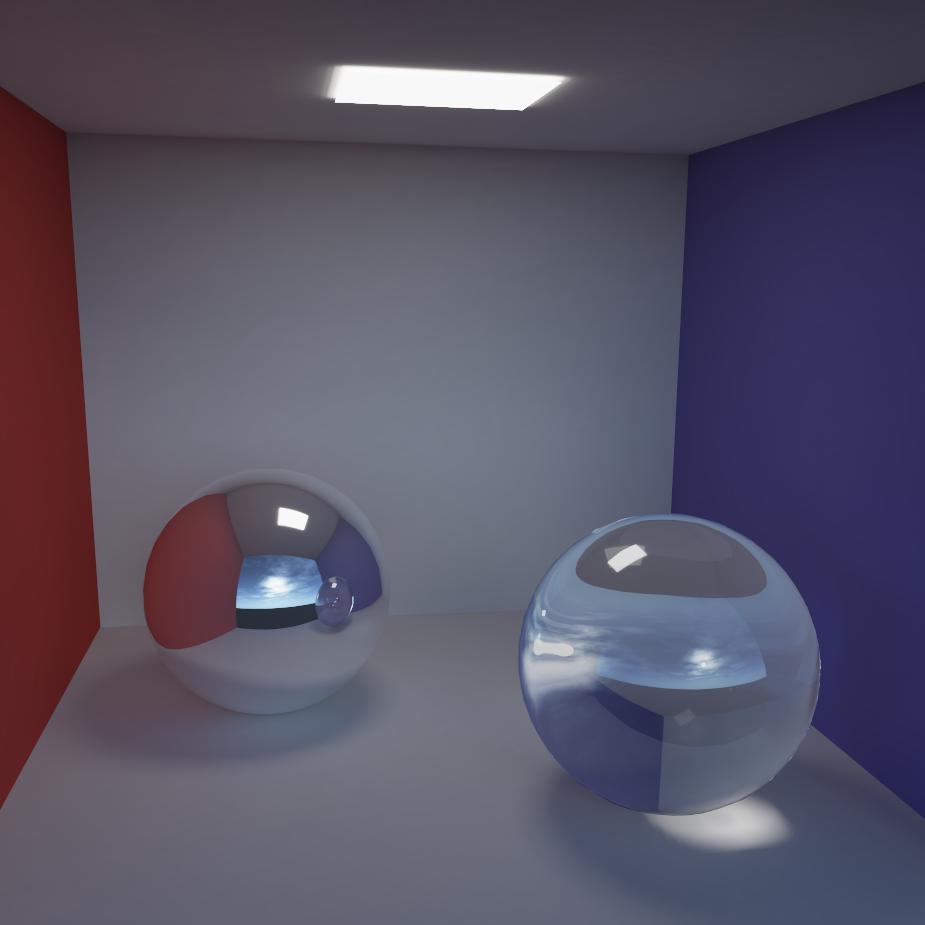
\includegraphics[width=0.95\textwidth]{pic/irrmap-cornell-irrmap.png}
			\caption{Irradiance Map}
		\end{subfigure}
		\caption[Irradiance-Map anhand der \enquote{Cornell Box}-Szene]{Die Bilder zeigen die Standardabweichungen der \enquote{Cornell Box}-Szene aus Abbildung \ref{fig:irr-est-rc-shaderball} entsprechend der Benennung aus Abbildung \ref{fig:irr-est-rc-dragon}. Vor allem Bereiche, die schwach von außen beleuchtet werden oder in Nischen liegen, weisen einen erhöhten Fehler auf. Die regelmäßigen Artefakte entstehen durch geringe Auflösung der Mesh in diesen Bereichen.}
		\label{fig:irr-map-cornell}
	\end{figure}

	\begin{figure}[h]
		\begin{subfigure}[b]{0.5\textwidth}
			\center
			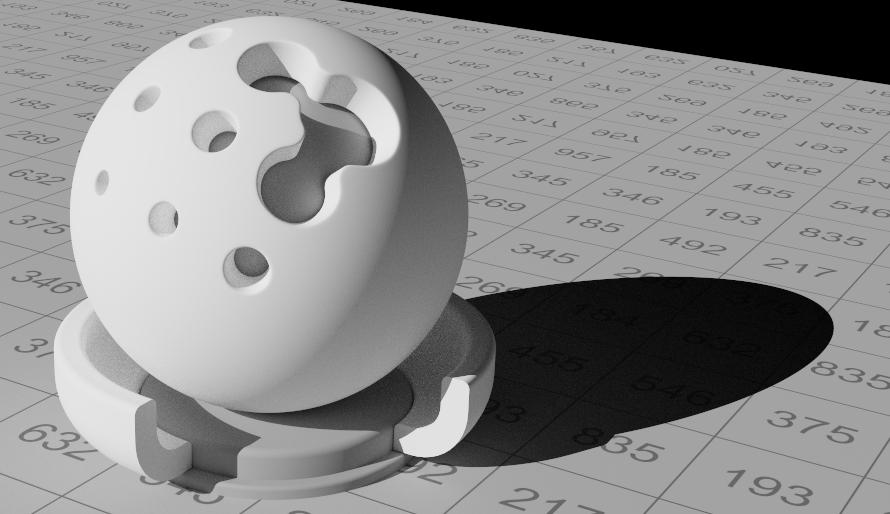
\includegraphics[width=0.95\textwidth]{pic/irrmap-shaderball-ref.png}
			\caption{Path Tracing}
		\end{subfigure}
		\begin{subfigure}[b]{0.5\textwidth}
			\center
			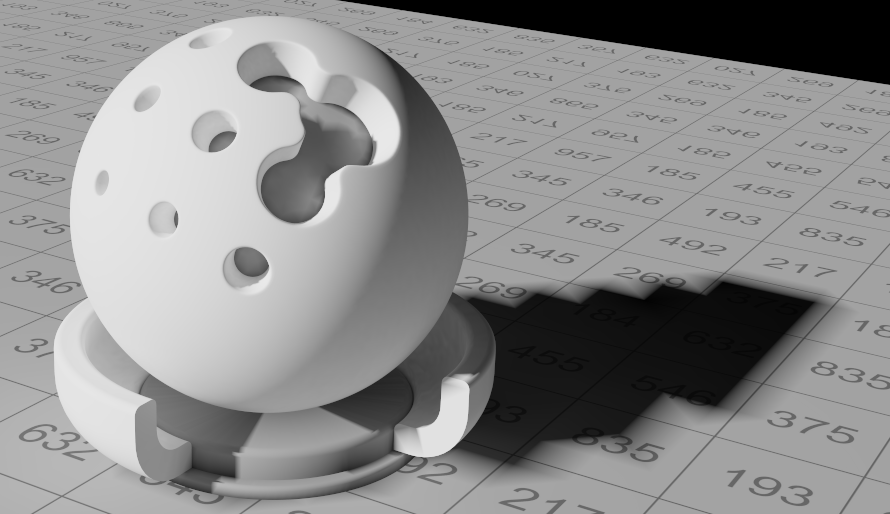
\includegraphics[width=0.95\textwidth]{pic/irrmap-shaderball-vmap.png}
			\caption{Vertex Lighting}
		\end{subfigure}
		\smallskip \\
		\begin{subfigure}[b]{0.5\textwidth}
			\center
			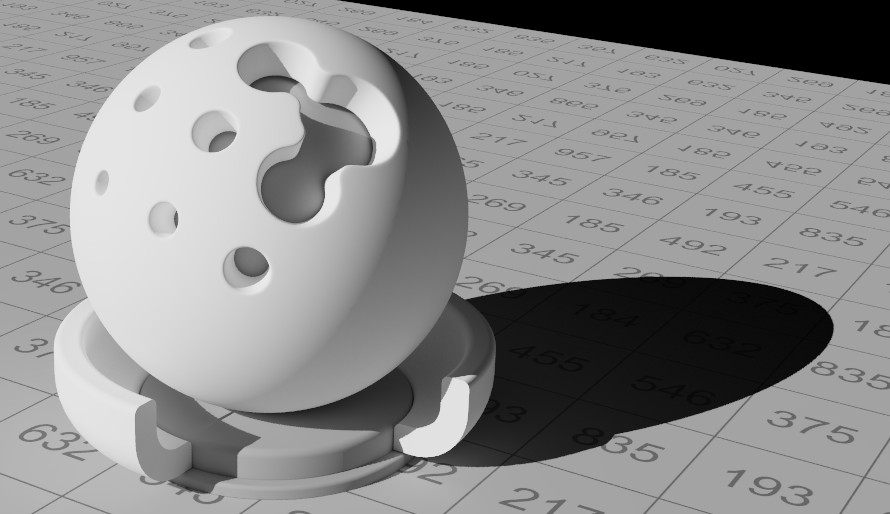
\includegraphics[width=0.95\textwidth]{pic/irrmap-shaderball-irrmap.png}
			\caption{Irradiance Map}
		\end{subfigure}
		\begin{subfigure}[b]{0.5\textwidth}
			\center
			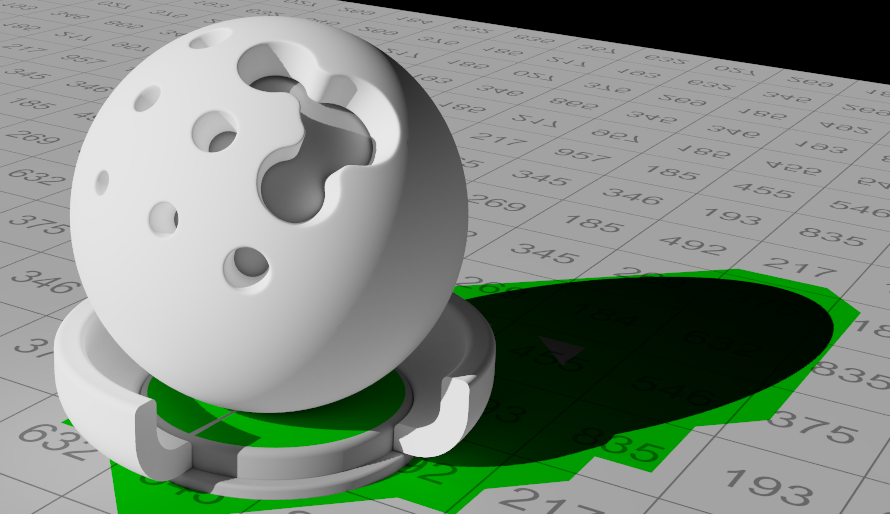
\includegraphics[width=0.95\textwidth]{pic/irrmap-shaderball-irrmap-order.png}
			\caption{Irradiance Map Ordnung}
		\end{subfigure}
		\caption[Irradiance-Map anhand der \enquote{Cornell Box}-Szene]{Die Bilder zeigen die Standardabweichungen der \enquote{Cornell Box}-Szene aus Abbildung \ref{fig:irr-est-rc-shaderball} entsprechend der Benennung aus Abbildung \ref{fig:irr-est-rc-dragon}. Vor allem Bereiche, die schwach von außen beleuchtet werden oder in Nischen liegen, weisen einen erhöhten Fehler auf. Die regelmäßigen Artefakte entstehen durch geringe Auflösung der Mesh in diesen Bereichen.}
		\label{fig:irr-map-cornell}
	\end{figure}

	\begin{figure}[h]
		\begin{subfigure}[b]{0.5\textwidth}
			\center
			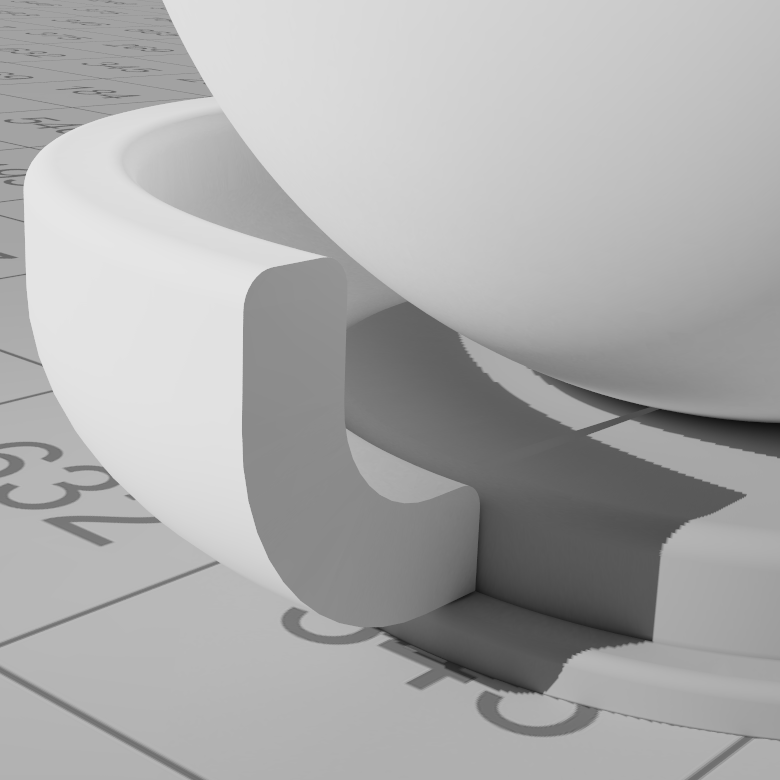
\includegraphics[width=0.95\textwidth]{pic/irrmap-shaderball2-irrmap.png}
			\caption{Irradiance Map}
		\end{subfigure}
		\begin{subfigure}[b]{0.5\textwidth}
			\center
			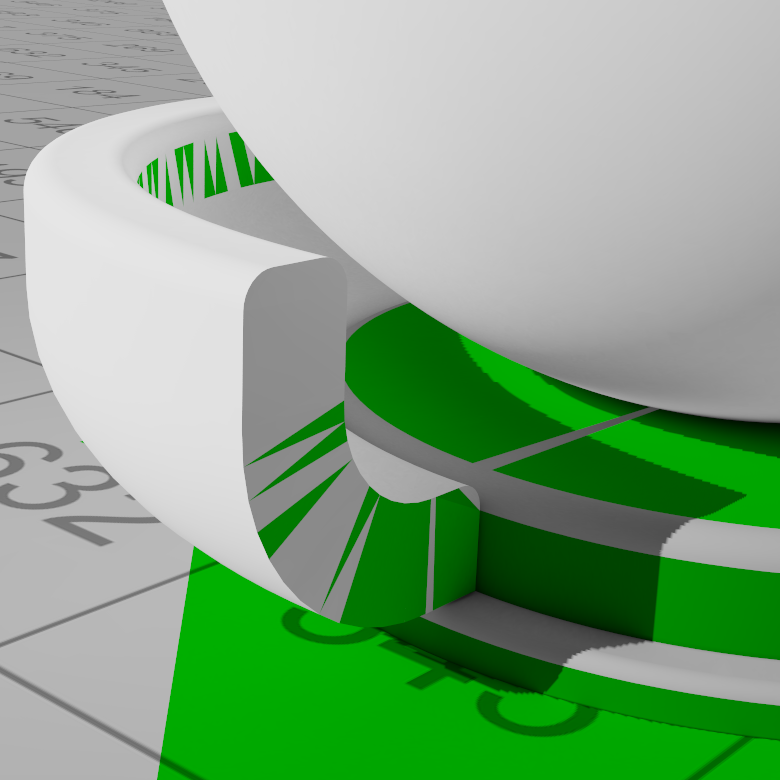
\includegraphics[width=0.95\textwidth]{pic/irrmap-shaderball2-irrmap-order.png}
			\caption{Irradiance Map Ordnung}
		\end{subfigure}
		\caption[Irradiance-Map anhand der \enquote{Cornell Box}-Szene]{Die Bilder zeigen die Standardabweichungen der \enquote{Cornell Box}-Szene aus Abbildung \ref{fig:irr-est-rc-shaderball} entsprechend der Benennung aus Abbildung \ref{fig:irr-est-rc-dragon}. Vor allem Bereiche, die schwach von außen beleuchtet werden oder in Nischen liegen, weisen einen erhöhten Fehler auf. Die regelmäßigen Artefakte entstehen durch geringe Auflösung der Mesh in diesen Bereichen.}
		\label{fig:irr-map-cornell}
	\end{figure}

	\medskip
\begin{tcolorbox}[colframe=black,colbacktitle=white,coltitle=black, attach boxed title to top center={yshift=-2mm},enhanced, titlerule=0.1pt, boxrule=0.5pt, arc=5pt,title=Quelltext:\quad Irradiance Map Generator, breakable]
	\lstinputlisting[style=std,language=c++]{code/gen_irr_map.cpp}
\end{tcolorbox}
\medskip

% section aufbau_und_generierung_der_irradiance_map (end)